% Main chapter title
\chapter{Anwendung}

% Chapter Label
\label{application}

In diesem Kapitel beschäftigen wir uns mit der Anwendung der dünnbesetzten Hauptkomponentenanalyse auf Frequenzdaten einer Mühle. Dafür stehen uns Zeitreihen von Beschleunigungssensoren, welche die Vibration der Maschine messen, sowie akustische Daten, welche durch Mikrofone aufgezeichnet werden, zur Verfügung. Wir sind interessiert daran herauszufinden, ob sich mithilfe der Zeitreihen Aussagen über die Partikelgröße des Materials treffen lassen. Aufgrund der Beschaffenheit des Datensatzes sind viele überwachte Lernverfahren in diesem Zusammenhang unbrauchbar. Im Zuge einer explorativen Analyse kann daher eine Dimensionsreduktion sinnvoll sein. Dabei sind wir nicht unbedingt an der niedrigdimensionalen Repräsentation der Daten interessiert, sondern viel mehr an der Herausfilterung wichtiger Frequenzen. Idealerweise erhalten wir eine Trennung der Frequenzen je nachdem, ob sie durch die Maschine oder durch das Material erzeugt worden sind. Die Möglichkeit der Interpretation und die Konsistenz waren Anlass für die Verwendung der dünnbesetzten Hauptkomponentenanalyse in diesem Zusammenhang. 

Zunächst werden wir dafür in Abschnitt \ref{data_set} den Datensatz näher beschreiben und Vorverarbeitungsschritte in \ref{prepros
} erläutern. Ergebnisse der Anwendung. Darüber hinaus werden wir die Wahl der Hyperparameter, die Laufzeit und die Korrektheit des Algorithmus in \ref{evaluation} thematisieren.

Ob eine derartige Methode für diesen Datensatz sinnvoll war, werden wir in Kapitel \ref{conclusion} diskutieren.


%----------------------------------------------------------------------------------------
%	Beschreibungs des Datensatzes
%----------------------------------------------------------------------------------------


\section{Beschreibung des Datensatzes}
\label{data_set}

Wir verfügen über Zeitreihen von Beschleunigungssensoren sowie Mikrofonen, die an unterschiedlichen Positionen einer Mühle angebracht sind. Um eine Trennung von Maschine und Material in den Daten zu ermöglichen, wurden Messungen sowohl mit als auch ohne Material durchgeführt. Des Weiteren wurden verschiedene Eigenschaften der Maschine verändert, was zu unterschiedlichen Mahlergebnissen führt. 

Durch eine hohe Abtastrate haben wir es mit einem hochdimensionalen Datensatz zu tun. Für jeden angebrachten Sensor haben wir somit $p \approx 5000000$ Zeitpunkte. Mit nur $n \approx 30$ Messungen, wobei Messungen mit Material mehrmals aufgezeichnet worden sind, sehen wir uns mit einer \textit{high dimension low sample size (HDLSS)} Situation konfrontiert. 

\section{Vorverarbeitung der Daten}
\label{preprocessing}

Vor der Anwendung der dünnbesetzten Hauptkomponentenanalyse auf den Datensatz haben wir einige Vorverarbeitungsschritte vorgenommen. Anfänglich sind uns wie beschrieben Zeitreihen gegeben. Da die Messungen zu zufälligen Zeitpunkten bei laufendem Mahlprozess gestartet worden sind, können einzelne Zeitpunkte nicht direkt miteinander verglichen werden. Mit einer Fouriertransformation der Daten können wir anstatt auf der Zeitachse auf den Frequenzen arbeiten, welche besser verglichen werden können. Zusätzlich erhofft man Rauscheffekte in dieser Darstellung besser zu erkennen. In Abbildung REF zeigen wir das Ergebnis einer Fouriertransformation beispielhaft für einen Sensor.

Es wird sich zeigen, dass der Algorithmus für die dünnbesetzte Hauptkomponentenanalyse sehr rechenintensiv sein kann. Daher haben wir uns entschieden, nur einen Teil der ursprünglichen Zeitreihe zu verwenden. Abbildung REF rechtfertigt diesen Schritt. Hier sieht man, dass sich die Frequenzen über die Zeit kaum ändern, was daran liegt, dass der Maschine konstant Material zugeführt wird. Somit können wir die Dimension um einen Faktor $100$ reduzieren ohne wichtige Informationen zu verlieren. Des Weiteren wurden Teile der Frequenzen, welche außerhalb des Frequenzbereichs des jeweiligen Sensors liegen, abgeschnitten. Zu Schluss haben wir die Daten ähnlich wie bei der klassischen Hauptkomponentenanalyse zentriert, um die Varianzen der verschiedenen Frequenzen vergleichbarer zu machen.


%----------------------------------------------------------------------------------------
%	Anwedung auf Frequenzdaten
%----------------------------------------------------------------------------------------


\section{Anwendung auf Frequenzdaten}
\label{application_frequency_data}

Unsere Implementierung ermöglicht verschiedene Modellparameter zu wählen. Für eine Beschränkung der Laufzeit setzen wir eine maximale Anzahl an Iterationen von $500$ und eine Toleranz von $10^{-4}$. Falls nach $500$ Iterationen die vorgegebene Toleranz noch immer nicht erreicht ist, werden wir dies im Folgenden kenntlich machen. Ein weiterer Parameter den es zu wählen gilt, ist die Anzahl zu berechnender Hauptkomponenten. Wie bereits in \ref{sparse_pca_theorems} beschrieben, wird dazu meist die klassische Hauptkomponentenanalyse verwendet. Wir haben uns für Analysezwecke dazu entschieden einen Durchlauf mit $2$ und einen mit $10$ Hauptkomponenten zu starten. Interessanter ist die Wahl der Hyperparameter $\lambda$ und $\alpha$, welche wesentlichen Einfluss auf die Ergebnisse besitzen. Für die Wahl von $\lambda$ haben wir einerseits mehrere Werte ausprobiert, als auch eine Rastersuche bezüglich der in \ref{choice_of_tuning_parameters} beschriebenen BIC-Kriterien durchgeführt. Dafür verwenden wir auf einer log-Skala gleichverteilte Werte im Bereich zwischen $10^{-7}$ und $10^0$. Dagegen wählen wir für das Verhältnis zwischen Lasso und Ridge-Bestrafung die Werte $[0.1, 0.5, 0.7, 0.9, 0.95, 0.99, 1]$. Mithilfe der Kreuzvalidierung kann dann ein bester Wert für $\alpha$ bestimmt werden. Es hat sich in den Anwendungen gezeigt, dass eine geeignete Liste für $\alpha$ mehr Werte nahe bei $1$ hat, da sich dort die größten Änderungen ergeben. Damit stärken wir den Lasso-Strafterm im Vergleich zum Ridge-Strafterm. (Minimieren wir zeitgleich über $\lambda$ und $\alpha$

Exemplarisch werden wir uns nun mit einem der akustischen und einem der Beschleunigungssensoren weiter beschäftigen. An dieser Stelle möchten wir erwähnen, dass wir die Sensoren getrennt betrachten, d.h. die dünnbesetzte Hauptkomponentenanalyse auf die Sensoren einzeln anwenden. Dies ist aufgrund der Unterschiedlichkeit der Sensoren sinnvoll. Um einen Vergleich zu ermöglichen, haben wir zeitgleich die klassische Hauptkomponentenanalyse auf den Datensatz angewandt. Wir möchten nun ausgewählte Ergebnisse vorstellen. 


%----------------------------------------------------------------------------------------
%	Auswertung der Ergebnisse
%----------------------------------------------------------------------------------------


\section{Auswertung der Ergebnisse}
\label{evaluation}

Im Rahmen dieser Arbeit können wir nun einen begrenzten Teil der Ergebnisse vorstellen. Wir geben einen großen Überblick über die verschiedenen Effekte und gehen gegebenenfalls weiter ins Detail.

Einmal step by step
Exemplarisch zeigen, dass wir dünnbesetzte Hauptachsen haben. Klare Trennung z.B. nach rotation speed. Erklärte Varianz dropt.

\begin{itemize}
\item Scree Plot Akkustik Sensor / Vibration
\item Zusammensetzung der ersten Hauptachse Akkustik / Vibration
\item PC Graph 
\end{itemize}

Wie verhält sich sparsity mit $\alpha$?
Allerdings dann auch Erklärte Varianz dropt.
erklärte Varianz mit $\alpha$ plot und BIC-Kriterium optimal

\textbf{Experimentelle Überprüfung der berechneten Varianzen}

In Abschnitt \ref{adjustment_of_variances} haben wir unterschiedliche Wege zur Berechnung der Hauptkomponenten und deren erklärte Varianz gezeigt. Um die Arbeit von Camacho et al. \cite{camacho} experimentell zu überprüfen, werden wir vier Kriterien definieren, welche auf den unterschiedlichen Vorgehensweisen basieren. Für jede dieser wird die Varianz der Residuen addiert und mit der Gesamtvarianz des Datensatzes normalisiert.
\begin{itemize}
\item TotQR: $\quad \frac{\sum_{j=1}^k R_{jj}^2 + \spur{\mat E^T\mat E}}{\spur{\mat X^T\mat X}} \quad$ (Vorgehensweies Zou et al.)
\item TotZB: $\quad \frac{\spur{\mat B \mat Z^T \mat Z \mat B^T} + \spur{\mat E^T\mat E}}{\spur{\mat X^T\mat X}} \quad$ (Vorgehensweise Camacho et al.)
\end{itemize}
Bezüglich der Notation haben wir uns an Abschnitt \ref{adjustment_of_variances} gehalten. Zwei weitere Kriterien TotQR* und TotZB* ergeben sich durch die Korrektur der Hauptkomponenten mit der Moore-Penrose-Inverse $\mat Z^* = \mat X \mat B^T (\mat B^T\mat B)^+$. Falls alle Vorgehensweisen korrekt sind, können wir erwarten, dass jedes Kriterium den Wert $1$ hat. In Abbildung \ref{total_variance_validation} haben wir die Kriterien für unsere Experimente berechnet. Klar zu sehen ist, dass ohne eine Korrektur mit der Moore-Penrose-Inversen beide Varianten für die Varianzberechnung im Allgemeinem falsch sind. Auch wenn wir die Hauptkomponenten korrigieren, liefert die QR-Zerlegung keine richtigen Ergebnisse. Nur TotZB* hat in allen Fällen den Wert $1$ und ist damit der korrekte Weg, Hauptkomponenten und Varianzen zu berechnen. Somit können wir die Erkenntnisse aus \cite{camacho} experimentell bestätigen.

\begin{figure}
\centering
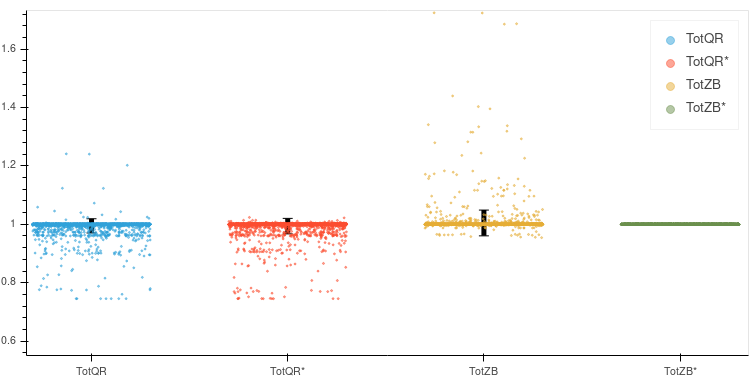
\includegraphics[width = 0.9\textwidth]{figures/total_variance_validation.png}
\caption{Zu sehen sind die Ergebnisse der unterschiedlichen Vorgehensweise bei der Berechnung der Hauptkomponenten und erklärter Varianzen. Nur die von Camacho et al. vorgeschlagene Variante TotZB* errechnet diese korrekt. Jeder Punkt entspricht eines unserer Experimente wie in Abschnitt \ref{application_frequency_data} beschrieben.}
\label{total_variance_validation}
\end{figure}

Laufzeit pro Iteration erhöht sich mit $\alpha$.
\begin{figure}
\centering
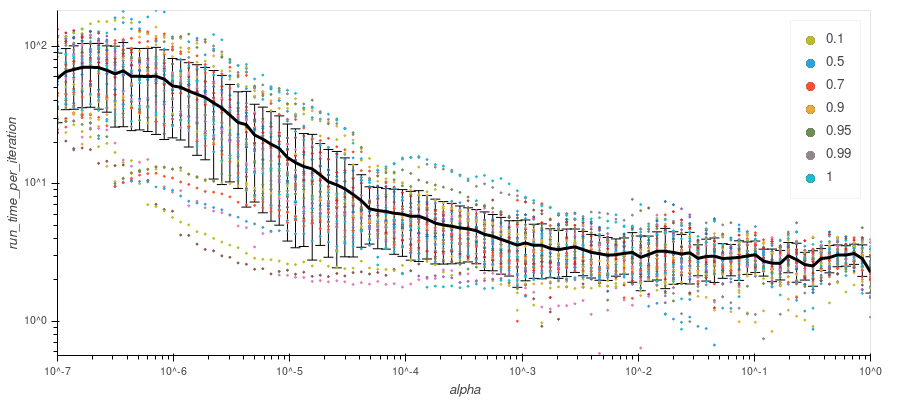
\includegraphics[width = 0.9\textwidth]{figures/run_time_per_iteration.png}
\caption{In dieser Abbildung ist die Laufzeit pro Iteration bei Veränderung des Hyperparameters $\lambda$ auf einer logarithmischen Skala zu sehen. Da auch $\alpha$ in unseren Experimenten variiert worden ist und mehrere Sensoren betrachtet werden, sehen wir mehrere Punkte je $\lambda$. Im Mittel klar zu erkennen ist ein Anstieg der Laufzeit bei Verringerung der Stärke der Bestrafung $\lambda$.}
\label{run_time_per_iteration}
\end{figure}

Anzahl an Iterationen mit $\alpha$?